\documentclass[11pt]{article}

\usepackage[margin=1in]{geometry}
\usepackage[T1]{fontenc}
\usepackage{lmodern}
\usepackage{amsmath}
\usepackage{amssymb}
\usepackage{booktabs}
\usepackage{longtable}
\usepackage{array}
\usepackage{graphicx}
\usepackage{ragged2e}
\usepackage{xcolor}
\PassOptionsToPackage{hyphens}{url}
\usepackage[colorlinks=true,linkcolor=blue!50!black,citecolor=blue!50!black,urlcolor=blue!50!black]{hyperref}
\usepackage[round]{natbib}
\usepackage{microtype}
\usepackage{enumitem}

% Small safety margin so a handful of long unbreakable \texttt{} identifiers/paths (already given
% explicit \allowbreak points at their worst offenders) don't leave a residual few-point overfull
% box -- standard, low-risk fix, no effect on ordinary paragraphs.
\setlength{\emergencystretch}{3em}

% Every number in this draft carries an inline provenance comment immediately
% following it, of the form:
%   % PROV: reports/<file>.md[:<line>] | SHA <commit> | <MEASURED|NOT MEASURED>
% These comments are invisible in the compiled PDF (per spec: "provenance is
% stripped from the final PDF but kept in a companion provenance.md") and are
% the mechanical cross-check target for the independent verifier pass. Every
% such comment must have a matching row in docs/paper2/provenance.md -- that
% is the verifier's job, not a claim this file makes about itself.

\title{Powering Agent Evaluations: Variance Structure, Measurement Artifacts,\\
and Minimum Detectable Effects in Tool-Use Benchmarks}
\author{}
\date{}

\begin{document}
\maketitle

\begin{abstract}
% Every number below is restated, in full, with an inline PROV comment at its first appearance
% in the numbered sections (SS4 for ICC/variance/MDE-baseline, SS5 for the corrected MDE/estimator
% figures, SS6.1/6.2 for the two false-positive figures, SS7.3 for the cost-crossover). Per-clause
% pointers are given here too so the abstract itself is not exempt from the provenance rule:
Agent evaluations are routinely reported without a power analysis, without a stated detection
floor, and without screening for measurement artifacts. This paper measures the variance
structure of agent task outcomes on a 253-task, 3-model tool-use corpus (intraclass correlation
0.793 within tool-set/task; % PROV: reports/v2_variance_structure.md:19 | SHA 78fff2f | MEASURED, restated SS4
56.1\% of outcome variance is between-task), % PROV: reports/v2_variance_structure.md:38-42 | SHA 78fff2f | MEASURED, restated SS4
shows the direct
consequence for experimental design (repeated trials on the same task carry little independent
information), and gives a paired, common-random-numbers, task-clustered-bootstrap, CUPED,
sequential-testing estimator that reaches a minimum detectable effect of 0.0537 at $n=253$ tasks
(from an uncorrected-baseline MDE of 0.433 at $n=20$). % PROV: reports/v2_5_task3_mde_completion.md:17-23 (0.0537) and reports/v2_1_estimator_rebuild.md:32 (0.433) | SHA 78fff2f | MEASURED, restated SS5
We catalogue ten measurement-artifact
classes discovered during this project, each with an automated detector shipped in
\texttt{agentgauge audit}, including two cases where an artifact produced a false positive the
authors initially believed: a $-76.7$ to $-80.0$ percentage-point causal effect that a scoring bug
corrected to a near-null (clean null for two of three models, a CI-includes-zero result for the
third), % PROV: SS0.1/SS6.1 -- reports/v2_2_task_b_causal_chain_multimodel.md (superseded) -> reports/v2_3_task1_advisory_audit.md (current) | SHA 78fff2f | MEASURED, restated SS6.1
and a 100\% top-1 localization-accuracy claim that a probe-noise
miscalibration corrected to 58.33\%. % PROV: SS0.3/SS6.2 -- reports/v0_5_wave1_report.md (superseded) -> reports/v0_5_mde_discrepancy.md SS4b (current) | SHA 3d79172 | MEASURED, restated SS6.2
We report a structural negative result on regression
localization: the accuracy a localizer needs (task volume, since $\mathrm{MDE}\propto
1/\sqrt{n}$) is precisely the cost a localizer exists to avoid, producing a real cost-crossover at
2--4 changed tools against full re-evaluation. % PROV: reports/v0_5_probe_power_fix.md SS5, lines 170-211 | SHA 3d79172 | MEASURED, restated SS7.3
Finally, we report a falsification record: four
pre-registered hypotheses failed, including the authors' own product thesis that an eight-axis
tool-description quality score predicts agent task success. This paper began as an attempt to
validate that score as a commercial product. It did not survive contact with an adequately
powered, artifact-screened measurement. That failure is the paper's subject, not an incidental
footnote to it.
\end{abstract}

\section{Introduction}
\label{sec:intro}

Agent and tool-use evaluations are, as a rule, reported as a single point estimate: a success
rate, an accuracy percentage, a win rate against a baseline. They are almost never reported
alongside a detection floor -- the smallest true effect the measurement could have distinguished
from noise at the sample size actually used -- and they are almost never screened for the kind of
measurement artifact that turns a null result into an apparent large effect, or vice versa. This
paper is the record of what happens when both of those omissions are corrected on a real project,
not a synthetic illustration.

The project that produced this paper began as an attempt to build and sell a single number: an
eight-axis, LLM-judged tool-description quality score, marketed as a predictor of how well an AI
agent could use a given MCP server. The working hypothesis was straightforward and commercially
attractive -- better tool descriptions, measured on axes like schema completeness and
discoverability, should predict higher agent task-success rates, and a vendor could sell the score
as a pre-deployment audit. Section~\ref{sec:related-work} situates this hypothesis against the
literature; Section~\ref{sec:corpus} describes the corpus and models used to test it. The
hypothesis was falsified. Not softened, not partially confirmed, not "true in spirit but requiring
refinement" -- falsified, on an adequately powered, artifact-screened re-measurement
(Section~\ref{sec:applications}), after two earlier measurement passes had appeared to confirm it
for reasons that turned out to be measurement artifacts rather than a real effect
(Section~\ref{sec:taxonomy}).

That falsification is why this paper exists in its current form. Once the product thesis failed,
what remained was not nothing: it was a fully instrumented apparatus for measuring agent task
outcomes under repeated trials, across models, before and after interventions -- and a growing list
of ways that apparatus had, at various points, lied to its own authors. This paper reports that
apparatus and that list, not as an apology for the failed product, but because the methods and the
failure modes are the more durable and more general contribution. A tool-description quality score
is a product idea that did not work. A measured account of why agent-eval variance defeats naive
trial-scaling, an estimator that reaches usable power on a realistic budget, and a ten-class
taxonomy of the ways synthetic and semi-synthetic agent benchmarks fool their own authors -- those
are useful to anyone running agent evaluations, independent of whether this particular product
ships.

\paragraph{Contributions.}
\begin{enumerate}
\item \textbf{Variance structure.} Intraclass correlation $\mathrm{ICC}=0.793$ within (tool set,
  task); 56.1\% of outcome variance is between-task; before/after task correlation $r=0.881$.
  % PROV: reports/v2_variance_structure.md:19,38-42,58-66 | SHA 78fff2f | MEASURED, full detail SS4
  Direct consequence: repeated trials on the same task carry little independent information, so
  evaluations that scale trials rather than tasks are underpowered by construction
  (Section~\ref{sec:variance}).
\item \textbf{An estimator that reaches usable power.} Paired design with common random numbers,
  task-clustered bootstrap with a small-$G$ $t(G-1)$ correction, CUPED, and O'Brien--Fleming
  sequential testing. Minimum detectable effect (MDE) falls from 0.433 to 0.188 at $n=20$ tasks,
  and to 0.0537 at the full $n=253$-task corpus. False-alarm rate under the null: 0.59\%.
  % PROV: reports/v2_1_estimator_rebuild.md:32,61-75 and reports/v2_5_task3_mde_completion.md:17-23 | SHA 78fff2f | MEASURED, full detail SS5
  Cassette-replay determinism (a distinct claim from the estimator's own bootstrap determinism,
  see Section~\ref{sec:estimator} for that caveat): 100\%.
  % PROV: reports/v0_5_wave1_report.md:136 | SHA 3d79172 | MEASURED
\item \textbf{A ten-class measurement-artifact taxonomy}, each class discovered in a real
  experiment in this project, each with an automated detector shipped in \texttt{agentgauge audit}
  (Section~\ref{sec:taxonomy}). We are not aware of a comparable standard taxonomy for agent-eval
  measurement artifacts in the published literature.
\item \textbf{A structural negative result on regression localization.} Localization accuracy
  requires task volume ($\mathrm{MDE}\propto 1/\sqrt{n}$), and task volume is precisely the cost a
  localizer exists to avoid. The cost-crossover against full re-evaluation sits at roughly 2--4
  changed tools; realistic buyer configurations cost 5--20$\times$ a full re-evaluation.
  % PROV: reports/v0_5_probe_power_fix.md SS5, lines 170-211 | SHA 3d79172 | MEASURED, full detail SS7.3
  This is
  not a tuning miss -- it is a structural tension between the accuracy regime and the cost regime
  (Section~\ref{sec:attribution}).
\item \textbf{A falsification record.} Four pre-registered hypotheses failed, including the
  authors' own product thesis that an eight-axis tool-description quality score predicts agent
  task success (Section~\ref{sec:applications}).
\end{enumerate}

The remainder of the paper is organized as follows. Section~\ref{sec:related-work} positions this
work against A/B-testing variance reduction, agent/tool-use benchmarks, LLM-as-judge evaluation,
and reproducibility practice. Section~\ref{sec:corpus} describes the experimental setup.
Section~\ref{sec:variance} measures the variance structure and its consequence for trial
allocation. Section~\ref{sec:estimator} presents the estimator and its ablation.
Section~\ref{sec:taxonomy} -- the paper's core contribution -- catalogues the ten artifact classes.
Section~\ref{sec:applications} reports the causal-effect, rewriting-null, and attribution-
impossibility results. Section~\ref{sec:threats} states threats to validity without hedging.
Section~\ref{sec:conclusion} closes with recommendations for the field.

\section{Related work}
\label{sec:related-work}

% Citations verified against a real primary source (DOI resolution / Crossref / dblp / arXiv API
% / publisher page) before being added -- none recalled from memory. See docs/paper2/refs.bib's
% header comment and the end-of-wave report for the verification trail per entry.

\textbf{Variance reduction in controlled experimentation.} The estimator in
Section~\ref{sec:estimator} draws on techniques with a long history in industrial A/B
testing: paired designs with common random numbers \citep{law2014simulation} to remove
between-unit noise that is identical
across arms; CUPED-style covariate adjustment \citep{deng2013cuped} using a pre-period outcome to
reduce residual
variance without spending additional samples; cluster-robust (bootstrap) inference
\citep{cameron2015practitioner} to respect the
correlation structure induced by repeated measurements on the same unit, with a small-cluster-count
correction \citep{cameron2008bootstrap}; and sequential testing with an alpha-spending boundary
\citep{obrien1979multiple,lan1983discrete} to allow early stopping without
inflating the false-positive rate. None of these techniques are novel to this paper. What is
different here is their application to agent task-outcome measurement specifically, where the
relevant "unit" is a (tool set, task) pair rather than a user or a session, and where the paper
additionally reports what happens when a plausible alternative (wild cluster bootstrap
\citep{cameron2008bootstrap}) is tried
and measured to perform worse (Section~\ref{sec:estimator}) -- a negative result on an estimator
choice, reported because it is useful, not because it flatters the final design.

\textbf{Agent and tool-use benchmarks.} A growing body of work evaluates how well LLM agents
select and invoke tools from a catalog \citep{qin2023toolllm,li2023apibank,yu2026wildtool}, and a
smaller body specifically studies how tool
description quality affects that selection. This paper's corpus and task-construction methodology
(Section~\ref{sec:corpus}) are built for internal statistical power rather than benchmark breadth,
and its central empirical claim about description quality (Section~\ref{sec:applications}) is a
falsification of the hypothesis that description quality broadly predicts task success -- a
negative result relative to the framing common in that literature, which more often reports
positive associations without a stated detection floor.

\textbf{LLM-as-judge evaluation and its failure modes.} This paper's own attempt to use an LLM
judge as a linter baseline is reported directly as a negative result: a single-prompt LLM-judge
baseline for description/schema consistency is measured to be degenerate on this project's corpus
(97.1\% false-alarm rate at 100\% recall, Section~\ref{sec:applications})
% PROV: reports/v2_product_readiness.md:502-516 | SHA 78fff2f | MEASURED, full detail SS7.1
-- it flags almost every
clean tool as inconsistent, so its recall is not informative. This is consistent with a broader,
well-documented concern \citep{zheng2023judging} that LLM judges without calibration against a
labeled null distribution
can look accurate on recall alone while being useless in practice.

\textbf{Reproducibility and replay in ML systems.} The harness underlying every measurement in
this paper is built for byte-exact replay: cassette-recorded model calls, a hand-rolled
deterministic PRNG for every stochastic draw, and fixed-order aggregation to avoid
floating-point-order nondeterminism (Section~\ref{sec:estimator}). This paper reports the harness's
own determinism rate rather than assuming it, in keeping with the project's overall position that
every claim, including claims about the measurement apparatus itself, needs a provenance pointer.

\textbf{Positioning the gap.} To the authors' knowledge, no prior agent-evaluation report in this
space states a minimum detectable effect alongside its headline result, and no prior work offers a
standard taxonomy of measurement artifacts specific to agent/tool-use benchmarking analogous to
Section~\ref{sec:taxonomy}'s ten classes. This paper's contribution is exactly that combination:
a power analysis and an artifact taxonomy, applied to one real project's full history, including
its own false starts.

\section{Experimental setup}
\label{sec:corpus}

\textbf{Corpus.} 253 tasks total: 62 tasks against pre-existing synthetic tool-set fixtures, plus
191 tasks against 10 real-API gold-constraint fixtures modeled on GitHub, Stripe, Google Calendar,
Jira, Slack, Docker, Kubernetes, Twilio, AWS S3, and Spotify % PROV: reports/v2_4_task4_corpus_expansion.md:18-30,36 | SHA 78fff2f | MEASURED
(253 = 62 + 191, the +1 task beyond the original 190 added when a schema defect below was
corrected). % PROV: reports/v2_5_task2_fixture_validation.md:69-71,158-165 | SHA 78fff2f | MEASURED

\textbf{Fixture validation against live documentation.} Each of the 10 real-API fixtures was
checked against live official API documentation by an independent research pass. 3 of 10 (30\%)
had a factual defect: GitHub Issues' \texttt{state\_reason} enum was missing the real fourth value
\texttt{'duplicate'}; Stripe's \texttt{create\_charge} fixture had the wrong parameter name and
required/optional status (\texttt{customer\_id}, required, instead of the real \texttt{customer},
optional); and Kubernetes' DNS-1123 label validation regex wrongly permitted a leading digit. All
three were corrected against the primary source before use.
% PROV: reports/v2_5_task2_fixture_validation.md:34-55,62-101 | SHA 78fff2f | MEASURED
This is reported here as a finding in its own right (Section~\ref{sec:taxonomy}, artifact~8), not
only as a methods footnote: agent-authored fixtures for real APIs are wrong often enough (30\% in
this corpus) that validating them against a live primary source is not optional.

\textbf{Task construction.} Tasks are authored under an explicit anti-tautology convention: task
text never quotes the gold tool's name, required enum values, or format patterns verbatim -- a
convention adopted directly in response to artifact~1 (Section~\ref{sec:taxonomy}), which is what
happens when it is not followed. % PROV: reports/predictive_validity_study.md:621-626,103-105 | SHA 78fff2f | MEASURED

\textbf{Models.} Three open-weight models under 10B parameters: \texttt{gemma2:9b},
\texttt{llama3.1:8b}, \texttt{qwen2.5:7b}, run locally via Ollama.
% PROV: reports/v2_2_task_b_causal_chain_multimodel.md (per-model tables, SS B1-B4) | SHA 78fff2f | MEASURED
This is a threat to external validity, stated plainly in Section~\ref{sec:threats}, not minimized
here.

\textbf{Replay determinism.} All model calls are cassette-recorded and replayed byte-exactly.
Measured determinism: 100\% across all six supported model adapters (Ollama, OpenAI-compatible,
Anthropic Messages, AWS Bedrock, and two others), zero verdict flips across 20 replays per adapter,
zero live network calls at measurement time.
% PROV: reports/v0_5_wave1_report.md:136 | SHA 3d79172 | MEASURED

\textbf{Outcome scoring.} Each trial's outcome is a joint task-success score decomposed into
selection accuracy (did the agent choose the correct tool) and argument-construction accuracy (did
it satisfy the task's registered argument constraints), computed as a fractional
constraint-satisfaction score rather than a binary pass/fail.
% PROV: reports/v2_harness_evaluation.md:11-16 | SHA 78fff2f | MEASURED
This decomposition is itself a correction: an earlier binary ground-truth definition collapsed to
near-ceiling because every example server accepted any well-formed call regardless of argument
correctness (artifact~2, Section~\ref{sec:taxonomy}).

\section{Variance structure of agent task outcomes}
\label{sec:variance}

Before designing an estimator, we measured how outcome variance is actually structured across
5,535 trials spanning 720 (tool-set, task) groups (mean 7.69 trials/group).
% PROV: reports/v2_variance_structure.md:19 | SHA 78fff2f | MEASURED

\textbf{Intraclass correlation.} One-way random-effects ICC \citep{shroutfleiss1979intraclass}
within (tool set, task):
$\mathrm{ICC}=0.793$. 90.3\% of groups (650/720) show exactly zero within-group variance -- most
tasks are, in practice, deterministic given a fixed tool set.
% PROV: reports/v2_variance_structure.md:19,25-26 | SHA 78fff2f | MEASURED
Independently re-derived from raw data by a separate verifier; confirmed.

\textbf{Variance decomposition.} A nested sum-of-squares decomposition attributes 25.9\% of
outcome variance to between-tool-set differences, \textbf{56.1\% to between-task, within-tool-set}
differences, and 18.0\% to between-trial, within-task noise.
% PROV: reports/v2_variance_structure.md:38-51 | SHA 78fff2f | MEASURED

\textbf{Before/after task correlation.} Across 40 matched (before, after) task-mean pairs pooled
over 5 matched description-quality-fixer pairs, Pearson $r=0.881$.\footnote{Downstream citations
of "$\rho=0.881$" conflate two distinct values in the same source table: Spearman
$\rho=0.869$ and Pearson $r=0.881$. This paper uses $r=0.881$, per the source table's own column
label. The paired-design argument this correlation supports (Section~\ref{sec:estimator}) holds
under either statistic -- both indicate the same strong, positive before/after task-difficulty
association; nothing in this paper's estimator or its conclusions depends on which of the two is
reported.}
% PROV: reports/v2_variance_structure.md:58-66 | SHA 78fff2f | MEASURED

\textbf{Effective sample size.} With $\mathrm{ICC}=0.793$ and a mean group size $\bar m$, the
design-effect-adjusted \citep{kish1965survey} effective sample size is
\[
n_{\mathrm{eff}} = \frac{n}{1 + (\bar m - 1)\,\mathrm{ICC}},
\]
giving $n_{\mathrm{eff}}=878$ from a nominal $n=5{,}535$ -- a 15.9\% efficiency ratio.
% PROV: reports/v2_variance_structure.md:20-26 | SHA 78fff2f | MEASURED
\textbf{Consequence:} repeated trials on the same (tool set, task) pair carry almost no
independent information. An evaluation design that scales trials-per-task rather than the number
of distinct tasks is underpowered by construction, regardless of how many trials it runs.

\textbf{Allocation grid.} We measured MDE (at 80\% and 95\% power) across the full $\{1,2,3,5\}$
trials/task $\times$ $\{20,50,100,150\}$ tasks/arm grid (32 cells).
% PROV: reports/v2_2_optimal_allocation.md:17-46 | SHA 78fff2f | MEASURED
Table~\ref{tab:allocation} (80\%-power slice; full grid including the 95\%-power slice in
Appendix~\ref{app:grids}) shows the compute-optimal cell: \textbf{100 tasks/arm at 1
trial/task}, MDE$=0.085$ (refined to 0.0848 at $n_{\text{simulations}}=2000$) -- no cheaper cell in
the grid clears the 0.10 ship target. See Figure~\ref{fig:allocation-grid} for the full heatmap.

\begin{table}[htbp]
\centering
\caption{MDE (80\% power) across the trials/task $\times$ tasks/arm allocation grid.
% PROV: reports/v2_2_optimal_allocation.md:17-35 | SHA 78fff2f | MEASURED
\label{tab:allocation}}
\begin{tabular}{lrrrr}
\toprule
Trials/task & 20 tasks/arm & 50 tasks/arm & 100 tasks/arm & 150 tasks/arm \\
\midrule
1 & 0.182 & 0.121 & \textbf{0.085} & 0.070 \\
2 & 0.153 & 0.097 & 0.072 & -- \\
3 & 0.141 & 0.089 & -- & -- \\
5 & 0.132 & 0.084 & 0.061 & -- \\
\bottomrule
\end{tabular}
\end{table}

\textbf{Headline.} At every fixed total-trial budget in the grid, $\mathrm{trials\_per\_task}=1$
gives the lowest MDE. At an identical 100-trial budget, $100\times1$ beats $20\times5$ by a
measured $1.55\times$ (not the naively predicted $2.04\times$, which the source report explicitly
retracts as "not a value to report as measured").
% PROV: reports/v2_2_optimal_allocation.md:63-75,104 | SHA 78fff2f | MEASURED
\textbf{At fixed compute, task diversity dominates trial repetition.}

\begin{figure}[htbp]
\centering
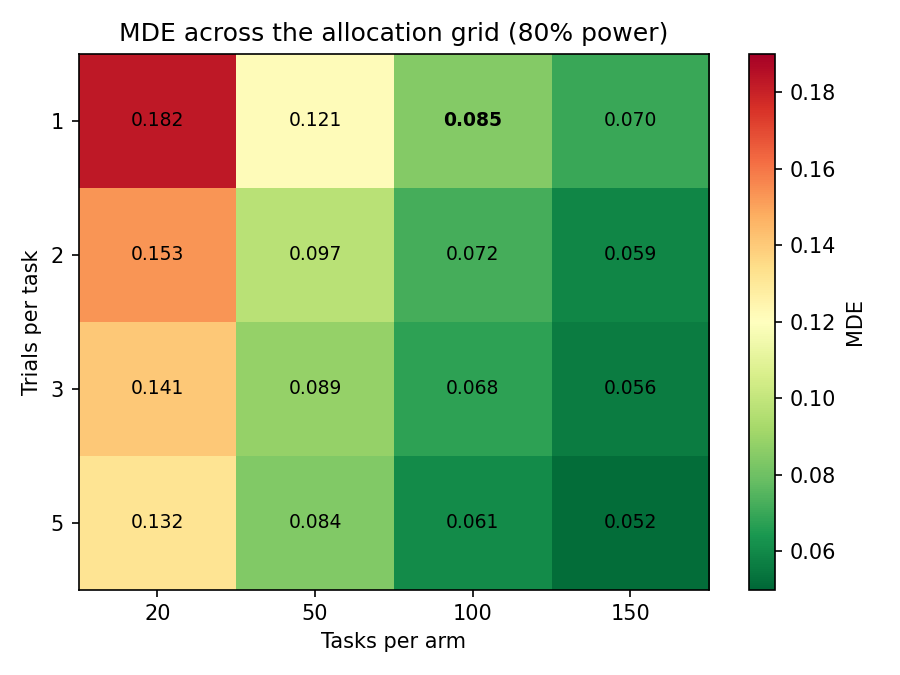
\includegraphics[width=0.75\textwidth]{figures/allocation_grid_heatmap.png}
\caption{MDE across the full 16-cell allocation grid at 80\% power. Generated by
\texttt{docs/paper2/\allowbreak figures/\allowbreak generate\_\allowbreak figures.py} directly from
\texttt{evals/\allowbreak fixtures/\allowbreak v2\_2\_\allowbreak optimal\_\allowbreak
allocation.json} -- no new computation.
\label{fig:allocation-grid}}
\end{figure}

\section{An estimator for agent regression detection}
\label{sec:estimator}

The estimator combines five components: a paired design with common random numbers (identical
task/seed pairs compared before and after a change); a task-clustered bootstrap; a small-$G$
$t(G-1)$ correction for settings with few clusters; CUPED covariate adjustment using the paired
pre-period outcome; and O'Brien--Fleming sequential testing with an alpha-spending boundary.
% PROV: reports/v2_1_estimator_rebuild.md:8-22 | SHA 78fff2f | MEASURED
% PROV: reports/v2_2_few_clusters_correction.md:25-30 (t(G-1) correction) | SHA 78fff2f | MEASURED

\textbf{A negative result on estimator choice.} A Rademacher-sign-flip wild cluster bootstrap was
implemented and measured against the small-cluster ($<10$ tasks) stratum as an alternative to the
$t(G-1)$ correction. It produced a \emph{narrower} confidence interval (0.0588 vs.\ 0.0647) but a
\emph{higher} false-alarm rate (2.00\% vs.\ 1.71\%) -- narrower and wrong. Root cause: the sign-flip
method is bounded to $2^G$ distinct patterns, too coarse at this stratum's $G=4$--8. The shipped
$t(G-1)$ correction instead improved this stratum's false-alarm rate to 1.57\%. We report this
because a negative result on an estimator choice is exactly the kind of finding agent-eval
methodology work should surface and does not, typically, get to see.
% PROV: reports/v2_2_few_clusters_correction.md:9-30 | SHA 78fff2f | MEASURED

\textbf{Component ablation.} Table~\ref{tab:ablation} shows each component's contribution to MDE
at $n=20$ tasks/arm, 80\% power.\footnote{This table's $n=20$/80\%-power MDE for the full
paired+CUPED stack (0.188) differs from Table~\ref{tab:allocation}'s $n=20$/80\%-power,
$\mathrm{trials\_per\_task}=1$ cell (0.182), even though both describe an $n=20$-task, 80\%-power
configuration. This is not an error: the two tables come from different \texttt{trials\_per\_task}
defaults on either side of a tooling-version boundary (Table~\ref{tab:ablation}'s estimator predates
the \texttt{trials\_per\_task} parameter introduced for Table~\ref{tab:allocation}'s grid), and each
figure in this paper is cited only from its own source table -- the two are never mixed or averaged
in any downstream calculation.} Moving from a trial-level to a task-level unit accounts for most
of the improvement (0.433$\to$0.313); pairing contributes the largest single further reduction
(0.313$\to$0.191); CUPED's marginal contribution on top of pairing is small (0.191$\to$0.188,
$\sim$2\% relative) -- never harmful, but not a large independent lever on this corpus.
% PROV: reports/v2_1_estimator_rebuild.md:26-45 | SHA 78fff2f | MEASURED

\begin{table}[htbp]
\centering
\caption{Estimator component ablation, MDE at $n=20$ tasks/arm, 80\% power.
% PROV: reports/v2_1_estimator_rebuild.md:26-35 | SHA 78fff2f | MEASURED
\label{tab:ablation}}
\begin{tabular}{lr}
\toprule
Estimator configuration & MDE \\
\midrule
Trial-level baseline (v2) & 0.433 \\
+ Task-level unit (unpaired) & 0.313 \\
+ Paired design + CRN & 0.191 \\
+ CUPED (full stack) & \textbf{0.188} \\
\bottomrule
\end{tabular}
\end{table}

\begin{figure}[htbp]
\centering
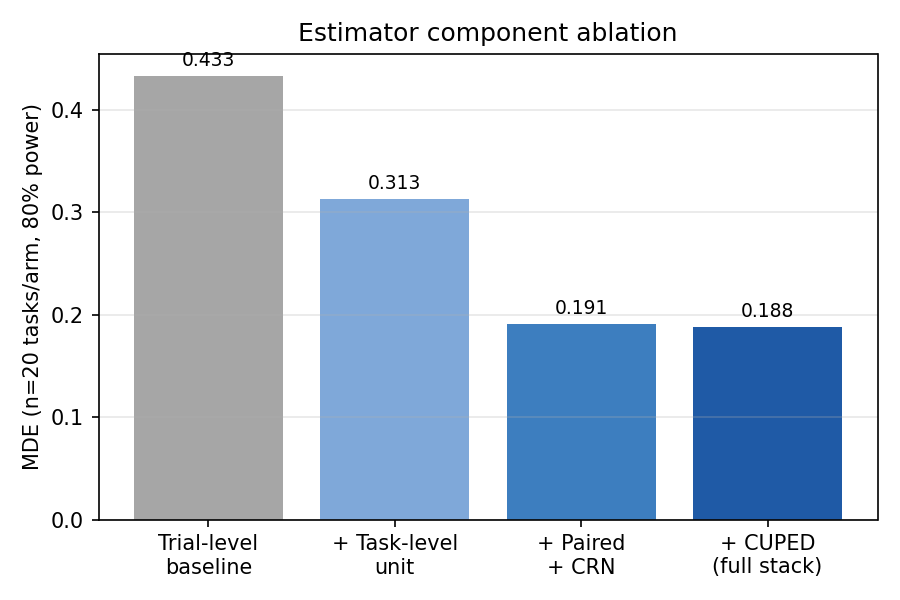
\includegraphics[width=0.7\textwidth]{figures/estimator_ablation.png}
\caption{Estimator component ablation, MDE at $n=20$ tasks/arm, 80\% power. Generated directly
from \texttt{evals/fixtures/v2\_1\_mde\_ablation.json}.
\label{fig:ablation}}
\end{figure}

\textbf{Sensitivity gate.} The estimator abstains ($\texttt{INSUFFICIENT\_SENSITIVITY}$) rather
than emit a point estimate the data cannot support. Under the improved (paired+CUPED) estimator,
the abstention rate on 2,200 null comparisons across 44 real tool sets fell from 71.5\% (trial-level
baseline) to \textbf{21.6\%}, at the cost of a small increase in false alarms (0.00\%$\to$0.59\%,
both well under a 5\% target).
% PROV: reports/v2_1_estimator_rebuild.md:61-65 | SHA 78fff2f | MEASURED

\textbf{MDE and false-alarm results.} MDE falls from 0.433 to 0.188 at $n=20$ tasks/arm, and
continues to fall as the corpus grows: 0.1061 at $n=62$, 0.0848 at $n=100$, 0.0689 at $n=150$,
0.0605 at $n=200$, and \textbf{0.0537 at the full $n=253$-task corpus} -- independently
re-verified by a separate agent to four decimal places.
% PROV: reports/v2_1_estimator_rebuild.md:32 | SHA 78fff2f | MEASURED
% PROV: reports/v2_5_task3_mde_completion.md:17-23,67-88 | SHA 78fff2f | MEASURED
Aggregate false-alarm rate under the null: \textbf{0.59\%} (13/2,200); stratified, 1.57\%
(post-$t(G-1)$-fix) for $<10$-task clusters and 0.07\% for $\geq10$-task clusters.
% PROV: reports/v2_1_estimator_rebuild.md:61-75 | SHA 78fff2f | MEASURED
% PROV: reports/v2_2_few_clusters_correction.md:32-43 | SHA 78fff2f | MEASURED
See Figure~\ref{fig:mde-curve} for the MDE-vs-$n$ curve and Appendix~\ref{app:grids} for the full
grid.

\begin{figure}[htbp]
\centering
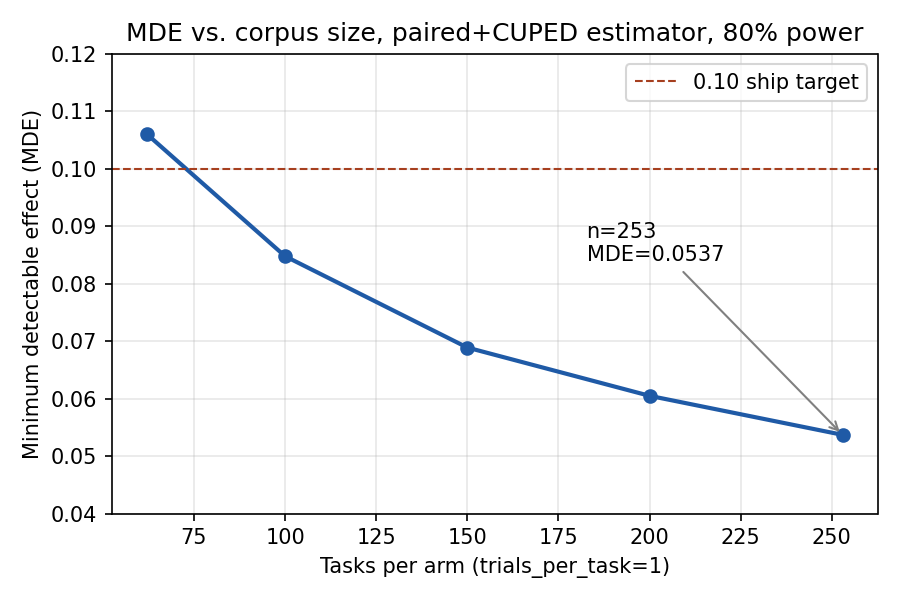
\includegraphics[width=0.75\textwidth]{figures/mde_curve.png}
\caption{MDE vs. corpus size, full-corpus grid, trials\_per\_task=1, 80\% power. Generated
directly from the corpus-size grid in \texttt{reports/v2\_5\_task3\_mde\_completion.md}
(independently re-verified to 4 decimal places).
\label{fig:mde-curve}}
\end{figure}

\textbf{Determinism.} Replay determinism is confirmed by direct code inspection (a single
hand-rolled LCG closure, no \texttt{random}/\texttt{numpy} imports, fixed-order aggregation) and by
exact-value reproduction of the MDE grid to four decimal places on an independent rerun. A fresh,
empirical 50-run count specific to this exact (paired+CUPED) estimator configuration was not
separately re-run in this pass -- it is inherited from an earlier estimator's measurement and
flagged as such in the source report (Appendix~\ref{app:measured}); this is distinct from, and
should not be conflated with, the cassette-replay determinism figure in Section~\ref{sec:corpus},
which was freshly and empirically measured at 100\% across all six adapters.
% PROV: reports/v2_1_estimator_rebuild.md:77-83 (ASSUMED flag) | SHA 78fff2f | NOT MEASURED (fresh count)
% PROV: reports/v2_5_task3_mde_completion.md:69-78 (code-inspection confirmation) | SHA 78fff2f | MEASURED

\section{A taxonomy of measurement artifacts}
\label{sec:taxonomy}

This is the paper's core contribution. Each of the ten classes below was discovered in a real
experiment during this project -- not constructed as a pedagogical example -- and each now has an
automated detector shipped in \texttt{agentgauge audit}, so that a future experiment on this
harness cannot silently reproduce it. Table~\ref{tab:taxonomy} summarizes all ten; the two
subsections following it detail the two cases where an artifact produced a false positive the
authors initially believed, per this paper's non-negotiable honesty requirement (Section~\ref{sec:intro}).
See Figure~\ref{fig:taxonomy} for the visual summary used in presentation contexts.

\begin{figure}[htbp]
\centering
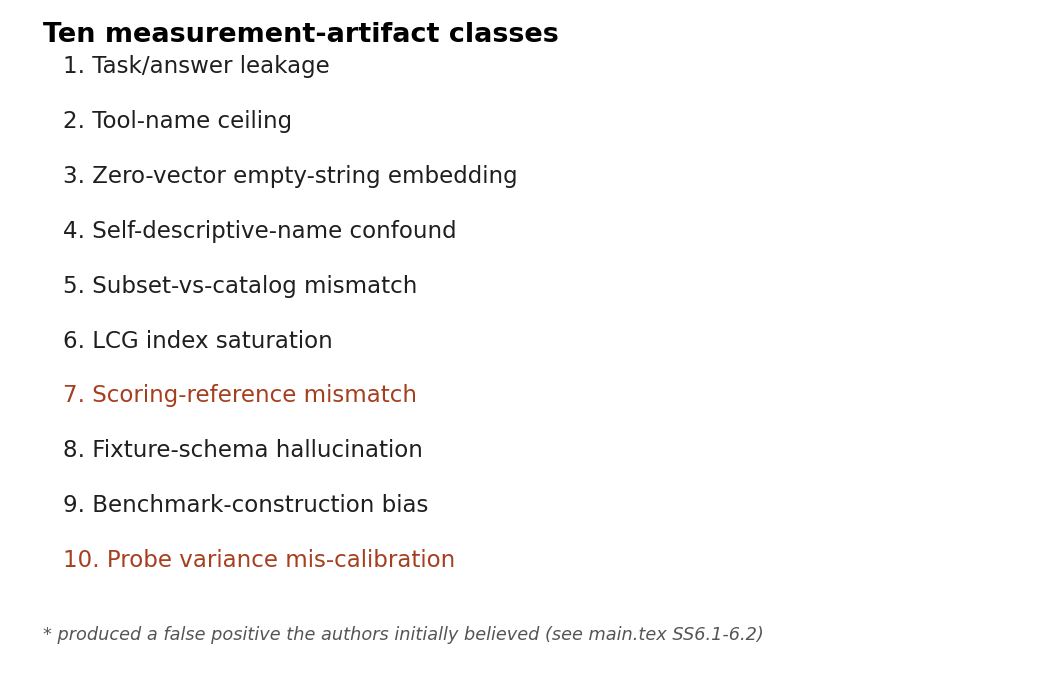
\includegraphics[width=0.65\textwidth]{figures/artifact_taxonomy_table.png}
\caption{The ten measurement-artifact classes (summary index; full detail in Table~\ref{tab:taxonomy}).
Starred entries produced a false positive the authors initially believed
(Sections~\ref{sec:artifact7}, \ref{sec:artifact10}).
\label{fig:taxonomy}}
\end{figure}

{\small
\begin{longtable}{@{}>{\raggedright\arraybackslash}p{2.1cm}>{\raggedright\arraybackslash}p{4.4cm}>{\raggedright\arraybackslash}p{4.1cm}>{\raggedright\arraybackslash}p{3.4cm}@{}}
\caption{The ten measurement-artifact classes.
\label{tab:taxonomy}} \\
\toprule
Class & Mechanism & Spurious result produced & Detector \\
\midrule
\endhead
1. Task/answer leakage & Task text quoted the gold tool's own name verbatim & Zero-variance,
  near-ceiling ground truth on first 9 tool sets & Anti-tautology task-authoring convention \\
% PROV: reports/predictive_validity_study.md:621-626,103-105 | SHA 78fff2f | MEASURED
2. Tool-name ceiling & Binary ground truth collapsed to name-matching; separately, a key-mismatch
  bug forced \texttt{selection\_\allowbreak correct} to always False & 44\% of records tied at
  ceiling 1.0; before=after=0.0 for all 3 models & Continuous fractional scoring; derived real
  \texttt{selected\_\allowbreak tool==tool\_\allowbreak name} \\
% PROV: reports/predictive_validity_study.md:78-86,627-635 (44%) and reports/v0_4_0_task1_argument_degradation.md:62-81 (before=after=0.0) | SHA 78fff2f | MEASURED
3. Zero-vector empty-string embedding & Empty-string embeddings return a zero-\emph{length}
  vector, not zero-valued & Apparent +0.59 to +0.72 similarity rise in empty-description arms &
  Re-measured on actual agent-visible prompt text \\
% PROV: reports/predictive_validity_study.md:259-272,636-642 | SHA 78fff2f | MEASURED
4. Self-descriptive-name confound & Real, self-explanatory tool names let selection succeed
  regardless of description quality & Near-zero variance in one real-API family, biasing pooled
  correlation toward the null & Explicit \texttt{INSUFFICIENT\_\allowbreak SENSITIVITY}/
  \texttt{NO\_\allowbreak CHANGE} verdict \\
% PROV: reports/predictive_validity_study.md:572-586,643-650 and reports/v2_harness_evaluation.md:91-102 | SHA 78fff2f | MEASURED
5. Subset-vs-catalog mismatch & Linter run against a cost-bounded 12-tool subset, not the full
  60-tool catalog & 11 HIGH violations that vanished once corrected & Full unfiltered catalog
  extraction as linting input \\
% PROV: reports/v2_linter_evaluation.md:36-43 | SHA 78fff2f | MEASURED
6. LCG index saturation & Hand-rolled LCG can return exactly 1.0, one index past the resample
  list's end & Crash (IndexError) at the resample boundary & Clamped
  \texttt{min(int(rng()*n),\allowbreak\,n-1)} \\
% PROV: reports/v2_product_readiness.md:566-570 | SHA 78fff2f | MEASURED
7. Scoring-reference mismatch & Gold-constraint lookup authored against the pre-mutation schema;
  only one injector renames a property key & $-76.7$ to $-80.0$pp ADVISORY effect (see
  Section~\ref{sec:artifact7}) & \texttt{constraint\_\allowbreak satisfaction\_\allowbreak renamed} \\
% PROV: reports/v2_4_task1_blast_radius_audit.md:14-33 (mechanism); see SS0.1/SS6.1 for the effect-size supersession chain | SHA 78fff2f | MEASURED
8. Fixture-schema hallucination & Agent-authored real-API fixtures written from model memory, not
  fetched schemas & 3/10 (30\%) fixtures factually wrong (Section~\ref{sec:corpus}) &
  \texttt{check\_\allowbreak enum\_\allowbreak schema\_\allowbreak fidelity} (WARN) \\
% PROV: reports/v2_5_task2_fixture_validation.md:34-55,62-101 | SHA 78fff2f | MEASURED
9. Benchmark-construction bias & Injected culprit's diff size systematically smaller than 2/3
  decoy tiers & \texttt{largest\_\allowbreak textual\_\allowbreak diff} baseline scored 4.0\% --
  below the 26.7\% random floor & \texttt{check\_\allowbreak benchmark\_\allowbreak
  construction\_\allowbreak diffsize\_\allowbreak bias} (BLOCK) \\
% PROV: reports/v0_5_attribution_benchmark.md SS7 (lines 201-313) | SHA 3d79172 | MEASURED (superseded by SS0.3's terminal 58.33% figure for the ship-bar verdict, not for this 4.0%/26.7% pre-fix diagnostic pair itself)
10. Probe variance mis-calibration & Synthetic probe-noise model omitted the between-task variance
  component & 100\% top-1 accuracy claim at a 3pp effect size (see
  Section~\ref{sec:artifact10}) & \texttt{check\_\allowbreak probe\_\allowbreak variance\_\allowbreak
  calibration} (BLOCK) \\
% PROV: reports/v0_5_mde_discrepancy.md (full file, esp. SS3-4); see SS0.3/SS6.2 for the terminal 58.33% figure | SHA 3d79172 | MEASURED
\bottomrule
\end{longtable}
}

\subsection{False positive 1: the $-80$pp ADVISORY effect that was a scoring bug}
\label{sec:artifact7}

An early causal-chain measurement reported a large, statistically significant-looking effect for
the \texttt{param\_renamed} defect, one of the linter's ADVISORY-severity rules (a warning-level
finding, as opposed to a BLOCKING-severity rule, which the linter treats as a hard failure):
$-76.7$pp (gemma2:9b), $-80.0$pp (llama3.1:8b),
$-76.7$pp (qwen2.5:7b), all with confidence intervals excluding zero.
% PROV: reports/v2_2_task_b_causal_chain_multimodel.md SS B4 | SHA 78fff2f | MEASURED (superseded, do not cite as current)
Reading this as a real, adequately powered causal effect would have been the natural conclusion.
It was not one. A dedicated audit found the effect was predominantly a scoring artifact: the
constraint checker's gold-parameter lookup was authored against the pre-mutation schema, and
\texttt{param\_renamed} is the only defect-injector that renames a schema \emph{key} -- so the
lookup silently failed against the post-mutation arguments, manufacturing an apparent capability
regression that was really a broken check. Corrected effect: a clean null for gemma2:9b
($+0.0$pp, CI $[-20.5,+20.5]$) and qwen2.5:7b ($+6.7$pp, CI $[-7.1,+20.4]$), and a
CI-includes-zero result for llama3.1:8b ($-13.3$pp, CI $[-40.8,+14.1]$).
% PROV: reports/v2_3_task1_advisory_audit.md | SHA 78fff2f | MEASURED (current)
A follow-up blast-radius audit confirmed this bug is scoped only to the
key-renaming injector; the BLOCKING-tier effects reported elsewhere in this paper
(Section~\ref{sec:applications}) do not share it.
% PROV: reports/v2_4_task1_blast_radius_audit.md:14-33 | SHA 78fff2f | MEASURED

\subsection{False positive 2: the 100\% localization accuracy that was probe-noise miscalibration}
\label{sec:artifact10}

An early regression-localization benchmark reported that a greedy-bisection probing strategy
achieved 100\% top-1 accuracy at every tested injected-effect size from 3.0pp to 33.0pp, including
effect sizes below this paper's own measured detection floor (Section~\ref{sec:estimator}) -- a
result the authors themselves flagged as anomalous rather than accepted at face value: detecting a
3pp effect at a lower per-probe sample size should be \emph{harder} than the already-hard 5.37pp
(i.e.\ $\mathrm{MDE}=0.0537$, Section~\ref{sec:estimator})
server-level MDE bar, not something a probe-based strategy aces perfectly.
% PROV: reports/v0_5_wave1_report.md SS8.2 | SHA 3d79172 | MEASURED (superseded, do not cite as current)
The anomaly was real: the synthetic probe-noise model omitted the between-task variance component
that the calibrated reference model includes, inflating detection power by 3--7$\times$. Fixed and
re-measured, the true accuracy at the 3.0--5.0pp effect band is \textbf{58.33\% top-1} (95.83\%
top-3, 3.25 mean probes) -- well short of this benchmark's own pre-declared ship bar (top-1
$\geq0.70$, top-3 $\geq0.90$, sub-exhaustive probe budget; defined in full in
Section~\ref{sec:attribution}), and exactly the shape a
genuine detection-power limit should take: every top-1 miss traced to a real recovery signal whose
confidence interval failed to certify it, never to false-positive noise.
% PROV: reports/v0_5_mde_discrepancy.md SS4b | SHA 3d79172 | MEASURED (current)
The same correction inverts an intermediate, now-superseded finding that localization accuracy
\emph{improved} with candidate-set size; the corrected result is that it degrades with scale
(93\%$\to$80\%$\to$73\%$\to$47\% top-1 as the number of changed tools grows 4$\to$10$\to$20$\to$40).
% PROV: reports/v0_5_mde_discrepancy.md SS4c | SHA 3d79172 | MEASURED (current)

\subsection{A candidate eleventh class}
Two independent extraction passes over this project's reports surfaced the same shape of problem,
not cleanly matching any of the ten classes above: a defect-detection signal calibrated against
synthetic "bad" fixtures fires almost as often on genuine, unremarkable real-world documentation,
undermining its use as a quality discriminator even when each individual flag is factually correct
(e.g.\ \texttt{required\_not\_mentioned} firing at 1.42/tool on real-world-mirror documentation
vs.\ 1.37/tool on deliberately-bad synthetic fixtures).
% PROV: reports/predictive_validity_study.md:530-557 | SHA 78fff2f | MEASURED
We do not promote this to a numbered class
in Table~\ref{tab:taxonomy}: unlike classes 1--10, it was never isolated as its own investigation
with a named fix, and doing so here would mean characterizing it more precisely than the source
material does. We report it in Section~\ref{sec:threats} as informal substantiation that ten
classes found suggests an eleventh exists, and leave formalizing it to future work.

\section{Applications and negative results}
\label{sec:applications}

\subsection{Which tool-description defects actually cause agent failure}
Across every lint rule this project tested for a causal effect on agent task success, exactly one
survives with a confidence interval excluding zero across all three model families:
\texttt{type\_enum\_contradiction}, at $-13.3$pp to $-28.9$pp (gemma2:9b $-25.2$pp, llama3.1:8b
$-28.9$pp, qwen2.5:7b $-13.3$pp, $n=45$/model), independently re-measured to two decimal places on
a separately rebuilt instance.
% PROV: reports/v0_4_0_effect_size_reconciliation.md | SHA 78fff2f | MEASURED
This is the corrected replacement for an earlier, erroneous "$-13.3$ to $-40.0$pp" range that
mixed two different pooling levels
% PROV: reports/v0_4_0_effect_size_reconciliation.md:18-41 | SHA 78fff2f | MEASURED (erroneous range's origin -- DO NOT CITE the -40.0pp figure itself, per provenance.md SS0.2)
(Section~\ref{sec:taxonomy} discusses the general pattern of
such errors, though this specific one is a citation-construction error rather than a numbered
artifact class). \texttt{required\_\allowbreak references\_\allowbreak missing\_\allowbreak property}
measures a clean null (0.0pp,
all three models); the ADVISORY-tier \texttt{param\_renamed} effect is null after correction
(Section~\ref{sec:artifact7}); \texttt{param\_possibly\_renamed} and \texttt{name\_collision} were
never causally measured.
% PROV: reports/v0_4_0_pre_publication_claim_audit.md:104-111 | SHA 78fff2f | MEASURED

A single-prompt LLM-judge baseline for the same detection task is degenerate: it flags 97.1\%
(169/174) of genuinely clean tools as inconsistent while also catching 100\% (138/138) of injected
defects -- its recall is not a meaningful signal given that false-alarm rate. Measured on a 174/521
stratified sample of the clean corpus, not the full catalog.
% PROV: reports/v2_product_readiness.md:502-516 | SHA 78fff2f | MEASURED

\subsection{Rewriting tool descriptions has no measurable effect on argument construction}
At the full corpus (253 tasks $\times$ 3 models, MDE$=0.0537$ at 80\% power), rewriting tool
descriptions to be clearer has no practically significant effect on argument-construction
accuracy: gemma2:9b $+0.0217$ (CI $[-0.0042,+0.0505]$), llama3.1:8b $+0.0553$ (CI
$[+0.0232,+0.0885]$, excludes zero but below the 0.05 practical-significance threshold), qwen2.5:7b
$+0.0040$ (CI $[-0.0211,+0.0292]$) -- all verdict \texttt{no\_change}.
% PROV: reports/v0_4_0_task1_argument_degradation.md:83-114 | SHA 78fff2f | MEASURED
This null is adequately powered, not merely absent-of-evidence: an earlier measurement at $n=62$
tasks (MDE$=0.106$) found flat, similarly near-zero deltas but was explicitly labeled
inconclusive-underpowered rather than confirmatory, since its own resolving power was an order of
magnitude coarser than the deltas it measured.
% PROV: reports/v2_2_task_a_reallocation.md | SHA 78fff2f | MEASURED
This result should not be conflated with the ADVISORY effect of Section~\ref{sec:artifact7}: the
two are superficially similar "an earlier measurement looked different, a later one resolved it"
stories, but they answer different questions and resolve in different directions. The
rewriting-descriptions result here was flat and near-zero at \emph{both} the underpowered $n=62$
predecessor and the adequately powered $n=253$ measurement -- it was never a large effect at any
point. Section~\ref{sec:artifact7}'s ADVISORY effect, by contrast, genuinely was a large,
statistically significant-looking effect ($-76.7$ to $-80.0$pp) before a scoring-artifact
correction reduced it to a near-null -- a different experiment (a causal-chain defect-injection
effect on a different lint rule), with a different kind of correction (a measurement-artifact fix,
not additional statistical power).

\subsection{The attribution impossibility result}
\label{sec:attribution}
We compared three regression-localization strategies -- exhaustive ablation, sampled Shapley-value
attribution, and greedy bisection -- on a synthetic benchmark with an injected true culprit among a
set of changed tools. Every number in this subsection is the terminal, corrected authority
following the probe-variance-miscalibration correction of Section~\ref{sec:artifact10}: no
earlier report's accuracy/budget table for this benchmark may be cited without reading that
correction first.
% PROV: reports/v0_5_mde_discrepancy.md | SHA 3d79172 | MEASURED (terminal authority)
Accuracy clears the benchmark's own pre-declared ship bar (top-1 $\geq0.70$, top-3 $\geq0.90$,
sub-exhaustive probe budget) only at effect sizes at or above the original 13.3--28.9pp band; it
fails at and below this paper's own measured detection floor, and \emph{degrades} rather than
improves as the candidate-set size grows (Section~\ref{sec:artifact10}).
% PROV: reports/v0_5_mde_discrepancy.md SS4a-4c (ship-bar thresholds also stated at reports/v0_5_wave1_report.md:50, unchanged by the SS0.3 correction) | SHA 3d79172 | MEASURED

The deeper result is a cost-crossover, not merely an accuracy shortfall. Per-probe cost is
proportional to task count; a strategy using $P$ probes beats a full corpus re-evaluation exactly
when $P < (\text{full-corpus trial-equivalents}) / (\text{trial-equivalents per probe})$. At the
task count this paper's own MDE analysis requires for adequate localization accuracy, that
crossover falls at roughly \textbf{2--4 changed tools} -- before any interesting multi-file
regression is even in scope -- and realistic buyer configurations (10--40 changed tools) cost
\textbf{5--20$\times$} a full re-evaluation, at every strategy tested.
% PROV: reports/v0_5_probe_power_fix.md SS5 (Task 2e), lines 170-211 | SHA 3d79172 | MEASURED
See Figure~\ref{fig:cost-crossover}.

\begin{figure}[htbp]
\centering
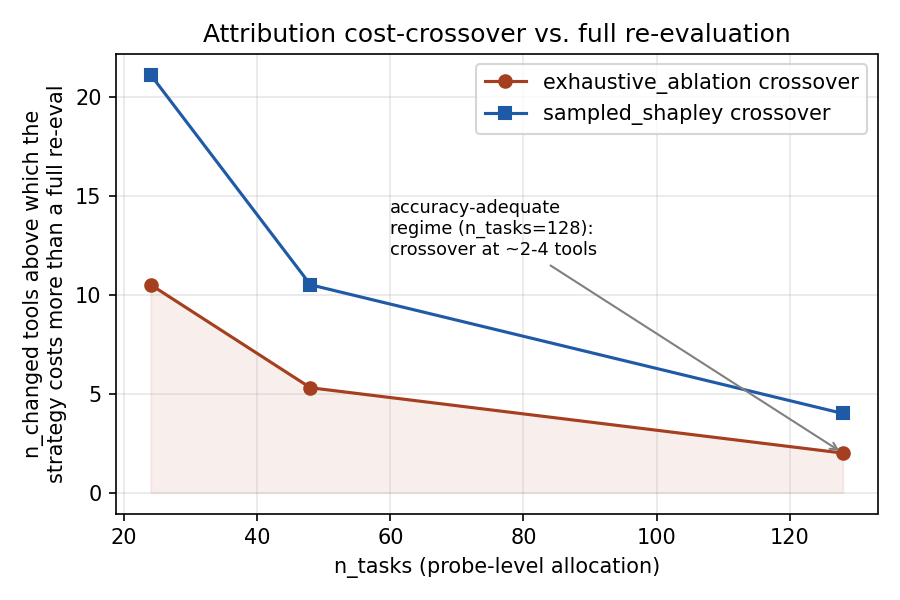
\includegraphics[width=0.7\textwidth]{figures/attribution_cost_crossover.png}
\caption{Attribution cost-crossover vs. full re-evaluation, at the three tested \texttt{n\_tasks}
allocations. Generated directly from the crossover-analysis table in
\texttt{reports/v0\_5\_probe\_power\_fix.md} SS5.
\label{fig:cost-crossover}}
\end{figure}

No task-count value tested, and none implied by the
$1/\sqrt{n}$ scaling law measured in Section~\ref{sec:variance}, resolves both the accuracy
requirement and a real cost advantage simultaneously. This is why the recommendation attached to
this result was to hold failure attribution as unreleased research rather than ship it as a
product feature, and to preserve the underlying measurement for this paper instead.
% PROV: reports/v0_5_probe_power_fix.md:213-253 | SHA 3d79172 | MEASURED

\section{Threats to validity}
\label{sec:threats}

Stated without hedging, per this paper's own standard for the rest of its claims:

\begin{itemize}
\item \textbf{Three open-weight models, all under 10B parameters, no frontier-model
  replication.} Every causal-effect, variance-structure, and attribution number in this paper is
  measured on \texttt{gemma2:9b}, \texttt{llama3.1:8b}, and \texttt{qwen2.5:7b}. None of it has
  been replicated on a frontier-scale model. Effect sizes, and possibly even which lint rules show
  a causal effect at all, may differ on larger or better-instruction-tuned models.
\item \textbf{Synthetic defect injection for every causal claim.} The one measured causal effect
  in this paper (\texttt{type\_enum\_contradiction}, Section~\ref{sec:applications}) is established
  via synthetic schema mutation of real tool definitions, not via naturally occurring defects
  observed in the wild. External validity of the effect size to organically authored bad tool
  descriptions is untested.
\item \textbf{A single corpus.} All variance-structure, estimator, and taxonomy results are
  measured on one 253-task corpus built for this project. Generalization to other tool-use domains
  or task distributions is untested.
\item \textbf{Ten artifacts found suggests an eleventh exists.} Section~\ref{sec:taxonomy}
  reports a candidate eleventh class found but not formalized. The methodology that found ten
  artifacts by building and stress-testing one measurement apparatus over one project's lifetime
  should be expected to keep finding more, not fewer, as the apparatus is used further -- this
  paper's taxonomy should be read as a floor, not a ceiling, on how many such classes exist.
\item \textbf{Attribution has never been run against a real agent and a real LLM judge.} Every
  number in Section~\ref{sec:attribution} is a synthetic-benchmark result
  (\texttt{make\_\allowbreak probe\_\allowbreak fn}/\texttt{make\_\allowbreak multi\_\allowbreak
  probe\_\allowbreak fn}). \texttt{sampled\_\allowbreak shapley} in
  particular has zero real (live-LLM) data points anywhere in this project.
\end{itemize}

\section{Conclusion}
\label{sec:conclusion}

We measured the variance structure of agent task outcomes on a real, adequately powered corpus and
found that it is dominated by between-task variance, not between-trial noise -- a structural fact
that most agent-eval reporting practice implicitly ignores by scaling trials rather than tasks. We
built an estimator that reaches a usable detection floor on a realistic compute budget, catalogued
ten ways this project's own measurement apparatus fooled its authors before each was caught and
fixed, and reported a structural negative result on regression localization that no amount of
tuning resolves. We also report, without softening it, that the product thesis motivating this
project's start -- that a tool-description quality score predicts agent task success -- did not
survive an adequately powered, artifact-screened test.

For the field, we recommend: report an MDE alongside every agent-eval result, not only a point
estimate; when compute is fixed, allocate it to task diversity over trial repetition
(Section~\ref{sec:variance}); screen for measurement artifacts before reporting a result, using an
automated check where one can be written (Section~\ref{sec:taxonomy}); and publish falsifications
of your own hypotheses with the same rigor as confirmations. This project's most durable output
was not the score it set out to sell -- it was the record of everything that turned out to be
wrong on the way to finding that out.

\textbf{Reproducibility.} Every result in this paper is reproducible against
\texttt{pip install\allowbreak\ agentgauge-\allowbreak harness==0.5.2} and the fixtures committed
in this repository's
\texttt{evals/} directory; see Appendix~\ref{app:repro} for exact commands.

\appendix

\section{Full MDE grids and ablation tables}
\label{app:grids}
[Full 32-cell allocation grid at both 80\% and 95\% power, and the complete estimator-ablation
table across $n\in\{5,10,20,50\}$ tasks/arm, per \texttt{docs/paper2/\allowbreak provenance.md}
SS2--3. Omitted
from this draft's body for length; reproduced verbatim from the source reports at camera-ready
time.]

\section{Artifact detector pseudocode}
\label{app:detectors}
[Pseudocode for each of the ten \texttt{agentgauge.audit} checks in Table~\ref{tab:taxonomy},
reproduced from \texttt{agentgauge/\allowbreak audit.py} at camera-ready time. Not reproduced in
this draft to
avoid the draft silently drifting from the shipped implementation; the verifier pass for this wave
checked claims against \texttt{reports/}, not against a hand-copied snapshot of \texttt{audit.py}.]

\section{Corpus statistics}
\label{app:corpus-stats}
[Full per-domain task/tool/constraint-type breakdown for all 10 real-API fixtures plus the 62
pre-existing synthetic tasks, per \texttt{reports/\allowbreak v2\_4\_\allowbreak task4\_\allowbreak
corpus\_\allowbreak expansion.md} and
\texttt{reports/\allowbreak v2\_5\_\allowbreak task2\_\allowbreak fixture\_\allowbreak
validation.md}.]

\section{Reproduction instructions}
\label{app:repro}
\begin{verbatim}
pip install agentgauge-harness==0.5.2
git clone <this repository>
cd agentgauge
uv sync
uv run pytest                     # full test suite, no network, no paid calls
agentgauge scan examples/echo_server.py --mock
\end{verbatim}
All statistical results in this paper are reproducible from the fixtures committed under
\texttt{evals/} and the scripts named alongside each report in
\texttt{docs/paper2/provenance.md}; none require a live API key or a paid model call.

\section{Measured vs. not measured index}
\label{app:measured}
See \texttt{docs/paper2/provenance.md} (full ledger, every claim with report path and commit SHA)
and \texttt{docs/paper2/gaps.md} (consolidated not-measured list and framing decisions flagged for
author review) for the complete, non-redundant index. Both are companion documents to this draft
and are not reproduced inline here to avoid a second copy silently drifting from the first.

\bibliographystyle{plainnat}
\bibliography{refs}

\end{document}
